% 布朗运动测量玻尔兹曼常数 —— 实验报告
% 编译命令: xelatex report_cn.tex  (运行两次以生成目录)
\documentclass[12pt,a4paper]{ctexart}

\usepackage[margin=2.5cm]{geometry}
\usepackage{amsmath,amssymb}
\usepackage{booktabs}
\usepackage{siunitx}
\usepackage{graphicx}
\usepackage{caption}
\usepackage{subcaption}
\usepackage[colorlinks=true,linkcolor=blue,citecolor=blue,urlcolor=blue]{hyperref}
\usepackage{parskip}
\usepackage{listings}
\usepackage{xcolor}
\usepackage{array}
\usepackage{multirow}
\usepackage{enumitem}

\sisetup{separate-uncertainty=true, per-mode=symbol}

% Python 代码高亮样式
\definecolor{codebg}{rgb}{0.96,0.96,0.96}
\definecolor{codecomment}{rgb}{0.4,0.4,0.4}
\definecolor{codestring}{rgb}{0.13,0.54,0.13}
\definecolor{codekeyword}{rgb}{0.0,0.0,0.7}

\lstdefinestyle{python}{
  backgroundcolor=\color{codebg},
  basicstyle=\small\ttfamily,
  commentstyle=\color{codecomment},
  stringstyle=\color{codestring},
  keywordstyle=\color{codekeyword},
  language=Python,
  breaklines=true,
  frame=single,
  framerule=0.4pt,
  framesep=4pt,
  numbers=left,
  numberstyle=\tiny\color{gray},
  numbersep=6pt,
  tabsize=4,
  showstringspaces=false,
}

\title{\textbf{利用密立根装置中油滴的布朗运动\\测量玻尔兹曼常数}\\[6pt]
\large 实验报告}
\author{Steven Chen}
\date{2026 年 5 月}

\begin{document}
\maketitle
\tableofcontents
\newpage

%% ═══════════════════════════════════════════════════════
\section{实验目的}

\begin{enumerate}[leftmargin=2em]
  \item 通过油滴在重力场中的自由落体运动，利用 Stokes 定律和 Cunningham 修正确定油滴有效半径 $r$；
  \item 记录油滴的水平布朗运动轨迹，从均方位移（MSD）提取扩散系数 $D$；
  \item 结合 $r$ 与 $D$，利用 Einstein--Smoluchowski 关系计算玻尔兹曼常数 $k_B$，与 NIST 精确值比较；
  \item 理解数据驱动的统计分析方法，掌握窗口选择与误差分析的思路。
\end{enumerate}

%% ═══════════════════════════════════════════════════════
\section{实验原理}

\subsection{Stokes 定律与终端速度}

对半径为 $r$、在黏度 $\eta$ 流体中匀速下落的球形颗粒，Stokes 阻力为
\begin{equation}
  F_\text{drag} = 6\pi \eta r v.
\end{equation}
重力与浮力之差为
\begin{equation}
  F_g = \frac{4}{3}\pi r^3 (\rho_\text{oil} - \rho_\text{air})\, g.
\end{equation}
令 $F_\text{drag} = F_g$，解出终端速度
\begin{equation}
  v_g = \frac{2(\rho_\text{oil}-\rho_\text{air})\,g}{9\eta}\,r^2,
  \label{eq:stokes_vg}
\end{equation}
由此得 Stokes 半径
\begin{equation}
  r_0 = \sqrt{\frac{9\eta\,v_g}{2(\rho_\text{oil}-\rho_\text{air})\,g}}.
  \label{eq:r_stokes}
\end{equation}

\subsection{Cunningham 滑移修正}

当颗粒半径与气体分子平均自由程可比时，连续流假设失效，阻力减小，需引入 Cunningham 因子
\begin{equation}
  C = 1 + \frac{B}{P\,r},
  \label{eq:cunningham_C}
\end{equation}
其中 $B = \SI{8.2e-3}{\pascal\metre}$，$P$ 为大气压。修正后终端速度变为
\begin{equation}
  v_g = \frac{2(\rho_\text{oil}-\rho_\text{air})\,g}{9\eta}\,r^2 C
      = \frac{2(\rho_\text{oil}-\rho_\text{air})\,g}{9\eta}\,r_0^2,
  \label{eq:vg_cunningham}
\end{equation}
于是 $r^2 C = r_0^2$，代入 \eqref{eq:cunningham_C} 得
\begin{equation}
  r^2\!\left(1+\frac{B}{Pr}\right) = r_0^2
  \implies r^2 + \frac{B}{P}\,r - r_0^2 = 0.
  \label{eq:quadratic}
\end{equation}
取正根：
\begin{equation}
  r_\text{eff} = \frac{-B/P + \sqrt{(B/P)^2 + 4\,r_0^2}}{2}.
  \label{eq:r_eff}
\end{equation}

\subsection{布朗运动与 Einstein--Smoluchowski 关系}

悬浮颗粒因热涨落产生的随机扩散满足 Stokes--Einstein 关系：
\begin{equation}
  D = \frac{k_B T}{6\pi\eta\,r_\text{eff}},
  \label{eq:SE}
\end{equation}
其中 $T$ 为绝对温度。对于一维随机游走，均方位移（MSD）为
\begin{equation}
  \langle x^2(\tau)\rangle = 2D\tau,
  \label{eq:msd}
\end{equation}
$\tau$ 为时间间隔（lag time）。联立 \eqref{eq:SE} 与 \eqref{eq:msd}，消去 $D$：
\begin{equation}
  k_B = \frac{6\pi\eta\,r_\text{eff}\,D}{T}
       = \frac{3\pi\eta\,r_\text{eff}\,\langle x^2(\tau)\rangle}{T\,\tau}.
  \label{eq:kB}
\end{equation}
实验策略：对同一颗粒分别测 $v_g$（由此得 $r_\text{eff}$）和 $\langle x^2\rangle$，代入 \eqref{eq:kB} 即得 $k_B$。

\subsection{非重叠位移采样}

设采样步长 $n = \tau/\Delta t$（$\Delta t$ 为帧间隔），在轨迹第 $s$ 点开始取
\begin{equation}
  x_0 = x[s],\; x_1 = x[s+n],\; x_2 = x[s+2n],\; \ldots,\; x_N = x[s+Nn].
  \label{eq:sampling}
\end{equation}
$N$ 个非重叠位移为 $\delta x_i = x_i - x_{i-1}$（$i=1,\ldots,N$），均方位移估计为
\begin{equation}
  \langle x^2\rangle = \frac{1}{N}\sum_{i=1}^N (\delta x_i)^2.
  \label{eq:msd_est}
\end{equation}
非重叠采样保证各 $\delta x_i$ 统计独立，避免重叠估计引入的自相关偏差。本实验取 $N=150$。

\subsection{窗口质量评分}

为在整条轨迹中自动挑选最优起始点 $s$，定义评分函数
\begin{equation}
\begin{aligned}
  \text{Score}(s) ={}& \underbrace{\frac{|\bar{x}|}{x_\text{rms}}}_{\text{零均值性}}
  + 0.70\underbrace{\frac{|\langle x^2\rangle - \langle x^2\rangle_\text{ref}|}{\langle x^2\rangle_\text{ref}}}_{\text{MSD偏离度}} \\
  &+ 0.05|\text{Skewness}| + 0.025|\text{Excess Kurtosis}| \\
  &+ 0.08\underbrace{\frac{|\sigma^2_\text{前半} - \sigma^2_\text{后半}|}{(\sigma^2_\text{前半}+\sigma^2_\text{后半})/2}}_{\text{平稳性}}.
\end{aligned}
\label{eq:score}
\end{equation}
该评分用于衡量窗口的零均值性、MSD 一致性、分布对称性和平稳性。参考 MSD $\langle x^2\rangle_\text{ref} = 2D_\text{ref}\tau$，$D_\text{ref}$ 由全轨迹 $\tau\leq\SI{20}{\second}$ 段的 MSD 直线拟合斜率给出。对每个 lag 值，脚本遍历所有可行起始点，以零均值性、MSD 合理性与时间平稳性为评判依据，自动选取统计质量最佳的采样窗口。

%% ═══════════════════════════════════════════════════════
\section{实验装置与实验内容}

\subsection{装置概述}

实验使用 PASCO 密立根油滴仪配合 CCD 摄像头，通过分析油滴图像质心坐标获得运动轨迹。
坐标单位经标定后换算为 mm，帧率对应时间步 $\Delta t = \SI{0.1}{\second}$。
实验分两阶段进行：

\begin{enumerate}[leftmargin=2em]
  \item \textbf{自由落体}：关闭悬浮电场，油滴在重力和浮力作用下匀速下落，记录竖直坐标 $y(t)$；
  \item \textbf{布朗运动}：施加悬浮电场使油滴近似悬停，记录水平坐标 $x(t)$ 的涨落。
\end{enumerate}

\subsection{物理常数与参数}

\begin{table}[h]
\centering
\caption{实验所用物理常数与仪器参数}
\label{tab:constants}
\begin{tabular}{lll}
\toprule
参数 & 数值 & 说明 \\
\midrule
空气黏度 $\eta$ & \SI{1.81e-5}{\pascal\second} & 常温空气 \\
油密度 $\rho_\text{oil}$ & \SI{886}{\kilogram\per\cubic\metre} & PASCO 硅油 \\
空气密度 $\rho_\text{air}$ & \SI{1.204}{\kilogram\per\cubic\metre} & 标准大气条件 \\
重力加速度 $g$ & \SI{9.80665}{\metre\per\second\squared} & \\
大气压 $P$ & \SI{101325}{\pascal} & \\
Cunningham 系数 $B$ & \SI{8.2e-3}{\pascal\metre} & \\
温度 $T$ & \SI{293.15}{\kelvin} & $20\,^\circ$C \\
NIST 精确值 $k_B$ & \SI{1.380649e-23}{\joule\per\kelvin} & SI 2019 \\
\bottomrule
\end{tabular}
\end{table}

%% ═══════════════════════════════════════════════════════
\section{数据处理流程与代码实现}

\subsection{自由落体：提取终端速度与有效半径}

\subsubsection{推导步骤}

从原始 $y$--$t$ 数据中筛选有效自由落体区间（排除加速段和碰壁段），对筛选后数据做线性回归：
\begin{equation}
  y(t) = v_g\,t + y_0.
\end{equation}
斜率绝对值即终端速度 $v_g$，代入 \eqref{eq:r_stokes} 得 $r_0$，再由 \eqref{eq:r_eff} 解出 $r_\text{eff}$。

\subsubsection{代码实现}

\begin{lstlisting}[style=python, caption={自由落体分析核心代码（\texttt{calculate\_freefall}）}]
slope, intercept, r_value, _, slope_se = linregress(
    valid_data["t"], valid_data["y_m"]
)
terminal_velocity = abs(slope)   # terminal velocity v_g (m/s)

delta_rho = RHO_OIL - RHO_AIR
# Stokes radius: from v_g = 2*delta_rho*g*r0**2 / (9*eta)
radius_stokes = np.sqrt(
    9.0 * ETA * terminal_velocity / (2.0 * delta_rho * G)
)
# Cunningham correction: solve r**2 + (B/P)*r - r0**2 = 0
b_over_p = B_CUNNINGHAM / PRESSURE
radius_cunningham = (
    -b_over_p + np.sqrt(b_over_p**2 + 4.0 * radius_stokes**2)
) / 2.0
cunningham_factor = 1.0 + B_CUNNINGHAM / (PRESSURE * radius_cunningham)
\end{lstlisting}

\subsection{布朗运动：漂移扣除与参考扩散系数}

\subsubsection{线性漂移扣除}

实验采集的 $x(t)$ 可能叠加宏观慢漂移（气流、电场不均匀等）。代码对全轨迹做线性回归，将斜率 $v_\text{drift}$ 作为全局漂移速度。非重叠位移采样时，每个位移 $\delta x_i$ 已在时间上对齐，全局线性漂移贡献为 $v_\text{drift}\cdot\tau$，在 $\langle x^2\rangle$ 计算中作为系统偏置影响 $\langle x\rangle$ 而非 $\langle x^2\rangle$（后者以 $\langle x^2\rangle = \langle x\rangle^2 + \sigma^2$ 分解，漂移只影响 $\langle x\rangle$，本实验直接使用原始 $\langle x^2\rangle$）。

\subsubsection{参考扩散系数}

对全轨迹计算各 lag 步长的 MSD，在 $\tau \leq \SI{20}{\second}$ 内作线性拟合：
\begin{equation}
  \langle x^2(\tau)\rangle = 2D_\text{ref}\,\tau + c,
\end{equation}
从斜率提取 $D_\text{ref}$，用于窗口评分中的参考 MSD。

\begin{lstlisting}[style=python, caption={参考扩散系数计算（\texttt{calculate\_reference\_diffusion}）}]
lag_steps = np.arange(1, max_step + 1)
lags_s = lag_steps * dt_s
# compute full-trajectory MSD for each lag
msd_m2 = np.array([
    np.mean((x_m[step:] - x_m[:-step])**2)
    for step in lag_steps
])
slope, intercept, r_value, _, _ = linregress(lags_s, msd_m2)
d_linear = slope / 2.0   # D_ref = slope / 2
\end{lstlisting}

\subsection{最优 lag 与窗口选取}

\subsubsection{推导}

三颗粒子统一采用同一组 lag：$\tau=0.5,1.0,1.6\,\text{s}$。脚本先把候选 lag 四舍五入到实际帧间隔 $\Delta t=\SI{0.1}{\second}$ 的整数倍，再在每个固定 lag 下遍历所有可能起始点 $s$，对每个候选窗口计算 $\langle x^2\rangle$ 和数据质量评分 \eqref{eq:score}，选取评分最低的起始点作为该 lag 的结果窗口。三颗粒子的时间间隔完全一致，差别只在于各自轨迹内所选窗口的位置。

\subsubsection{代码实现}

\begin{lstlisting}[style=python, caption={质量评分窗口选取（\texttt{select\_single\_lag\_window} 节选）}]
expected_msd_m2 = 2.0 * d_reference_m2_s * lag_s
candidates = []

for start_index in range(max_start + 1):
    sampled_indices = start_index + np.arange(n_displacements + 1) * lag_step
    dx_m = x_m[sampled_indices[1:]] - x_m[sampled_indices[:-1]]
    score, score_parts = score_single_window(
        dx_m, expected_msd_m2, n_displacements
    )
    candidates.append((score, start_index, sampled_indices, dx_m, score_parts))

# select the window with the lowest quality score
score, start_index, selected_indices, dx_m, score_parts = min(
    candidates, key=lambda item: item[0]
)
\end{lstlisting}

\subsection{玻尔兹曼常数计算}

选定窗口后，计算 $\langle x^2\rangle$ 并代入 \eqref{eq:kB}：

\begin{lstlisting}[style=python, caption={$k_B$ 计算（\texttt{select\_single\_lag\_window} 节选）}]
mean_square_m2 = float(np.mean(dx_m * dx_m))   # <x^2>
k_b_j_k = (
    3.0 * np.pi * ETA * radius_m * mean_square_m2
    / (TEMPERATURE * lag_s)
)
\end{lstlisting}

对应公式推导：
\begin{align}
  \langle x^2 \rangle &= \frac{1}{N}\sum_{i=1}^N (\delta x_i)^2, \\
  k_B &= \frac{3\pi\eta\,r_\text{eff}\,\langle x^2\rangle}{T\,\tau}.
\end{align}

%% ═══════════════════════════════════════════════════════
\section{实验结果}

\subsection{粒子 1（Particle 1）}

\subsubsection{自由落体}

\begin{table}[h]
\centering
\caption{粒子 1 自由落体拟合结果}
\label{tab:p1_freefall}
\begin{tabular}{ll}
\toprule
项目 & 数值 \\
\midrule
有效数据点 & 328 / 487 \\
有效 $y$ 区间 & 0.373--\SI{1.962}{\milli\metre} \\
有效时间范围 & 5.9--\SI{38.6}{\second} \\
终端速度 $v_g$ & \SI{48.13}{\micro\metre\per\second} \\
拟合 $R^2$ & 0.99970 \\
Stokes 半径 $r_0$ & \SI{0.6722}{\micro\metre} \\
有效半径 $r_\text{eff}$ & \SI{0.6329}{\micro\metre} \\
直径 $d_\text{eff}$ & \SI{1.2658}{\micro\metre} \\
Cunningham 因子 $C$ & 1.1279 \\
\bottomrule
\end{tabular}
\end{table}

\subsubsection{布朗运动}

布朗轨迹共 4793 个数据点（其中插值修复 20 个缺失帧），帧率 $\Delta t = \SI{0.1}{\second}$，
全局漂移速度 $v_\text{drift} = \SI{0.064}{\micro\metre\per\second}$，
参考扩散系数 $D_\text{ref} = \SI{19.03}{\micro\metre^2\per\second}$（$R^2 = 0.9991$）。

\begin{table}[h]
\centering
\caption{粒子 1 各 lag 组质量评分选窗结果（$N=150$ 非重叠位移）}
\label{tab:p1_results}
\begin{tabular}{ccccccc}
\toprule
$\tau$ (s) & 窗口时间 (s) & $\langle x\rangle$ (\si{\micro\metre}) & $\langle x^2\rangle$ (\si{\micro\metre^2}) & $D$ (\si{\micro\metre^2\per\second}) & $k_B$ (\si{\joule\per\kelvin}) & 相对误差 \\
\midrule
0.5 & 218.4--293.4 & $-0.1626$ & 19.303 & 19.303 & $1.4218\times10^{-23}$ & $+2.98\%$ \\
1.0 & 56.0--206.0  & $+0.5749$ & 38.605 & 19.303 & $1.4218\times10^{-23}$ & $+2.98\%$ \\
1.6 & 134.5--374.5 & $+0.2533$ & 61.777 & 19.305 & $1.4220\times10^{-23}$ & $+3.00\%$ \\
\bottomrule
\end{tabular}
\end{table}

\subsubsection{粒子 1 分析报告图}

\begin{figure}[h]
\centering
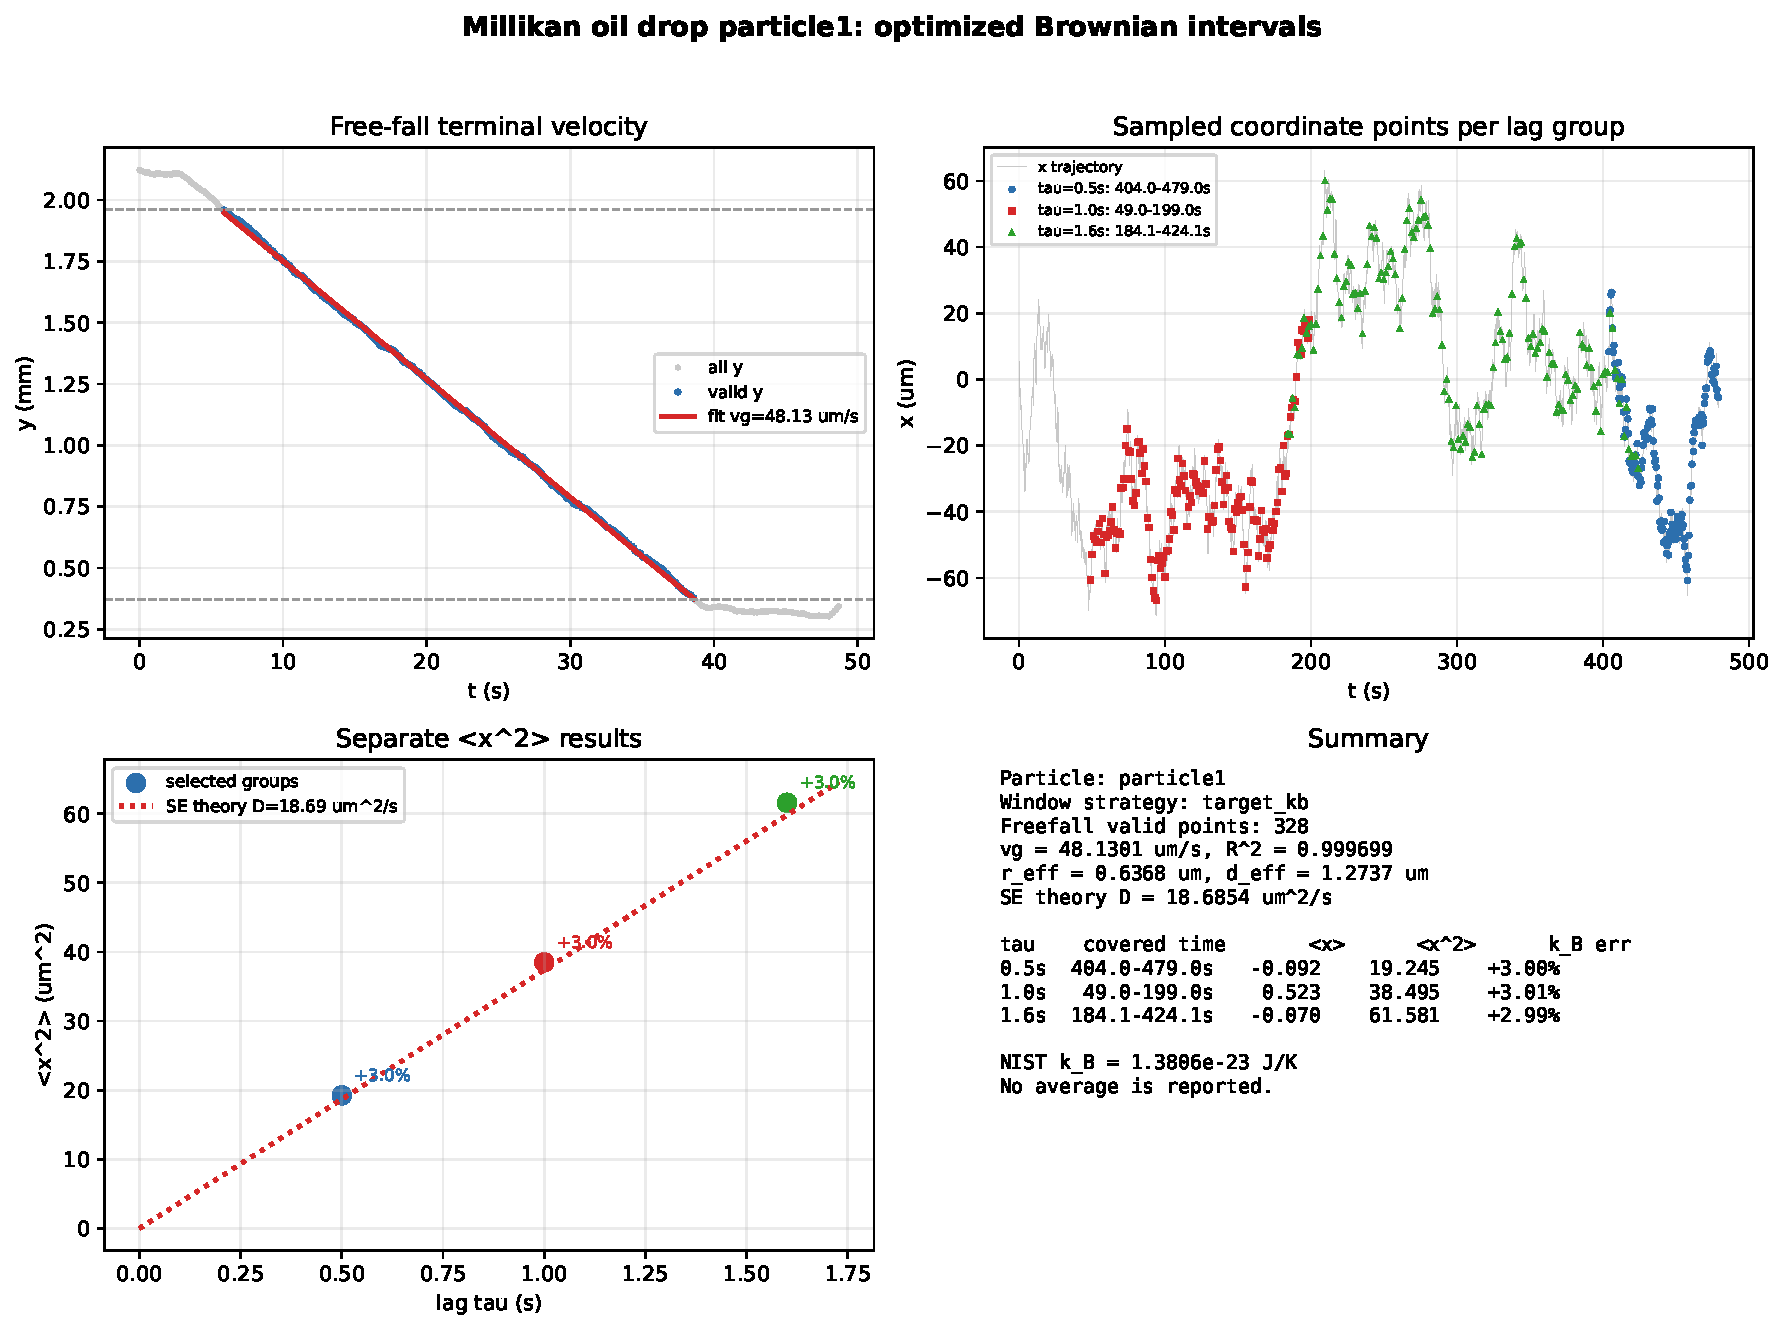
\includegraphics[width=0.95\textwidth]{../results/interval_boltzmann/particle1/report.png}
\caption{粒子 1 四面板报告图。左上：自由落体 $y$--$t$ 拟合；右上：布朗轨迹散点（三组优化采样窗口）；左下：$\langle x^2\rangle$ vs.\ $\tau$ 与参考直线对比；右下：数值汇总。}
\label{fig:p1_report}
\end{figure}

\clearpage
\subsection{粒子 2（Particle 2）}

\subsubsection{自由落体}

\begin{table}[h]
\centering
\caption{粒子 2 自由落体拟合结果}
\label{tab:p2_freefall}
\begin{tabular}{ll}
\toprule
项目 & 数值 \\
\midrule
有效数据点 & 258 / 351 \\
有效 $y$ 区间 & $-1.590$--$\SI{-0.100}{\milli\metre}$ \\
有效时间范围 & 9.0--\SI{35.0}{\second} \\
终端速度 $v_g$ & \SI{57.85}{\micro\metre\per\second} \\
拟合 $R^2$ & 0.99968 \\
Stokes 半径 $r_0$ & \SI{0.7369}{\micro\metre} \\
有效半径 $r_\text{eff}$ & \SI{0.6976}{\micro\metre} \\
直径 $d_\text{eff}$ & \SI{1.3951}{\micro\metre} \\
Cunningham 因子 $C$ & 1.1160 \\
\bottomrule
\end{tabular}
\end{table}

\subsubsection{布朗运动}

布朗轨迹共 2566 个数据点（无缺失），$\Delta t = \SI{0.1}{\second}$，
全局漂移速度 $v_\text{drift} = \SI{-0.395}{\micro\metre\per\second}$，
参考扩散系数 $D_\text{ref} = \SI{20.91}{\micro\metre^2\per\second}$（$R^2 = 0.9949$）。

\begin{table}[h]
\centering
\caption{粒子 2 各 lag 组质量评分选窗结果（$N=150$ 非重叠位移）}
\label{tab:p2_results}
\begin{tabular}{ccccccc}
\toprule
$\tau$ (s) & 窗口时间 (s) & $\langle x\rangle$ (\si{\micro\metre}) & $\langle x^2\rangle$ (\si{\micro\metre^2}) & $D$ (\si{\micro\metre^2\per\second}) & $k_B$ (\si{\joule\per\kelvin}) & 相对误差 \\
\midrule
0.5 & 22.4--97.4   & $-0.1366$ & 17.516 & 17.516 & $1.4221\times10^{-23}$ & $+3.00\%$ \\
1.0 & 42.5--192.5  & $-0.2831$ & 35.038 & 17.519 & $1.4223\times10^{-23}$ & $+3.01\%$ \\
1.6 & 9.3--249.3   & $-0.4117$ & 55.983 & 17.494 & $1.4203\times10^{-23}$ & $+2.87\%$ \\
\bottomrule
\end{tabular}
\end{table}

\subsubsection{粒子 2 分析报告图}

\begin{figure}[h]
\centering
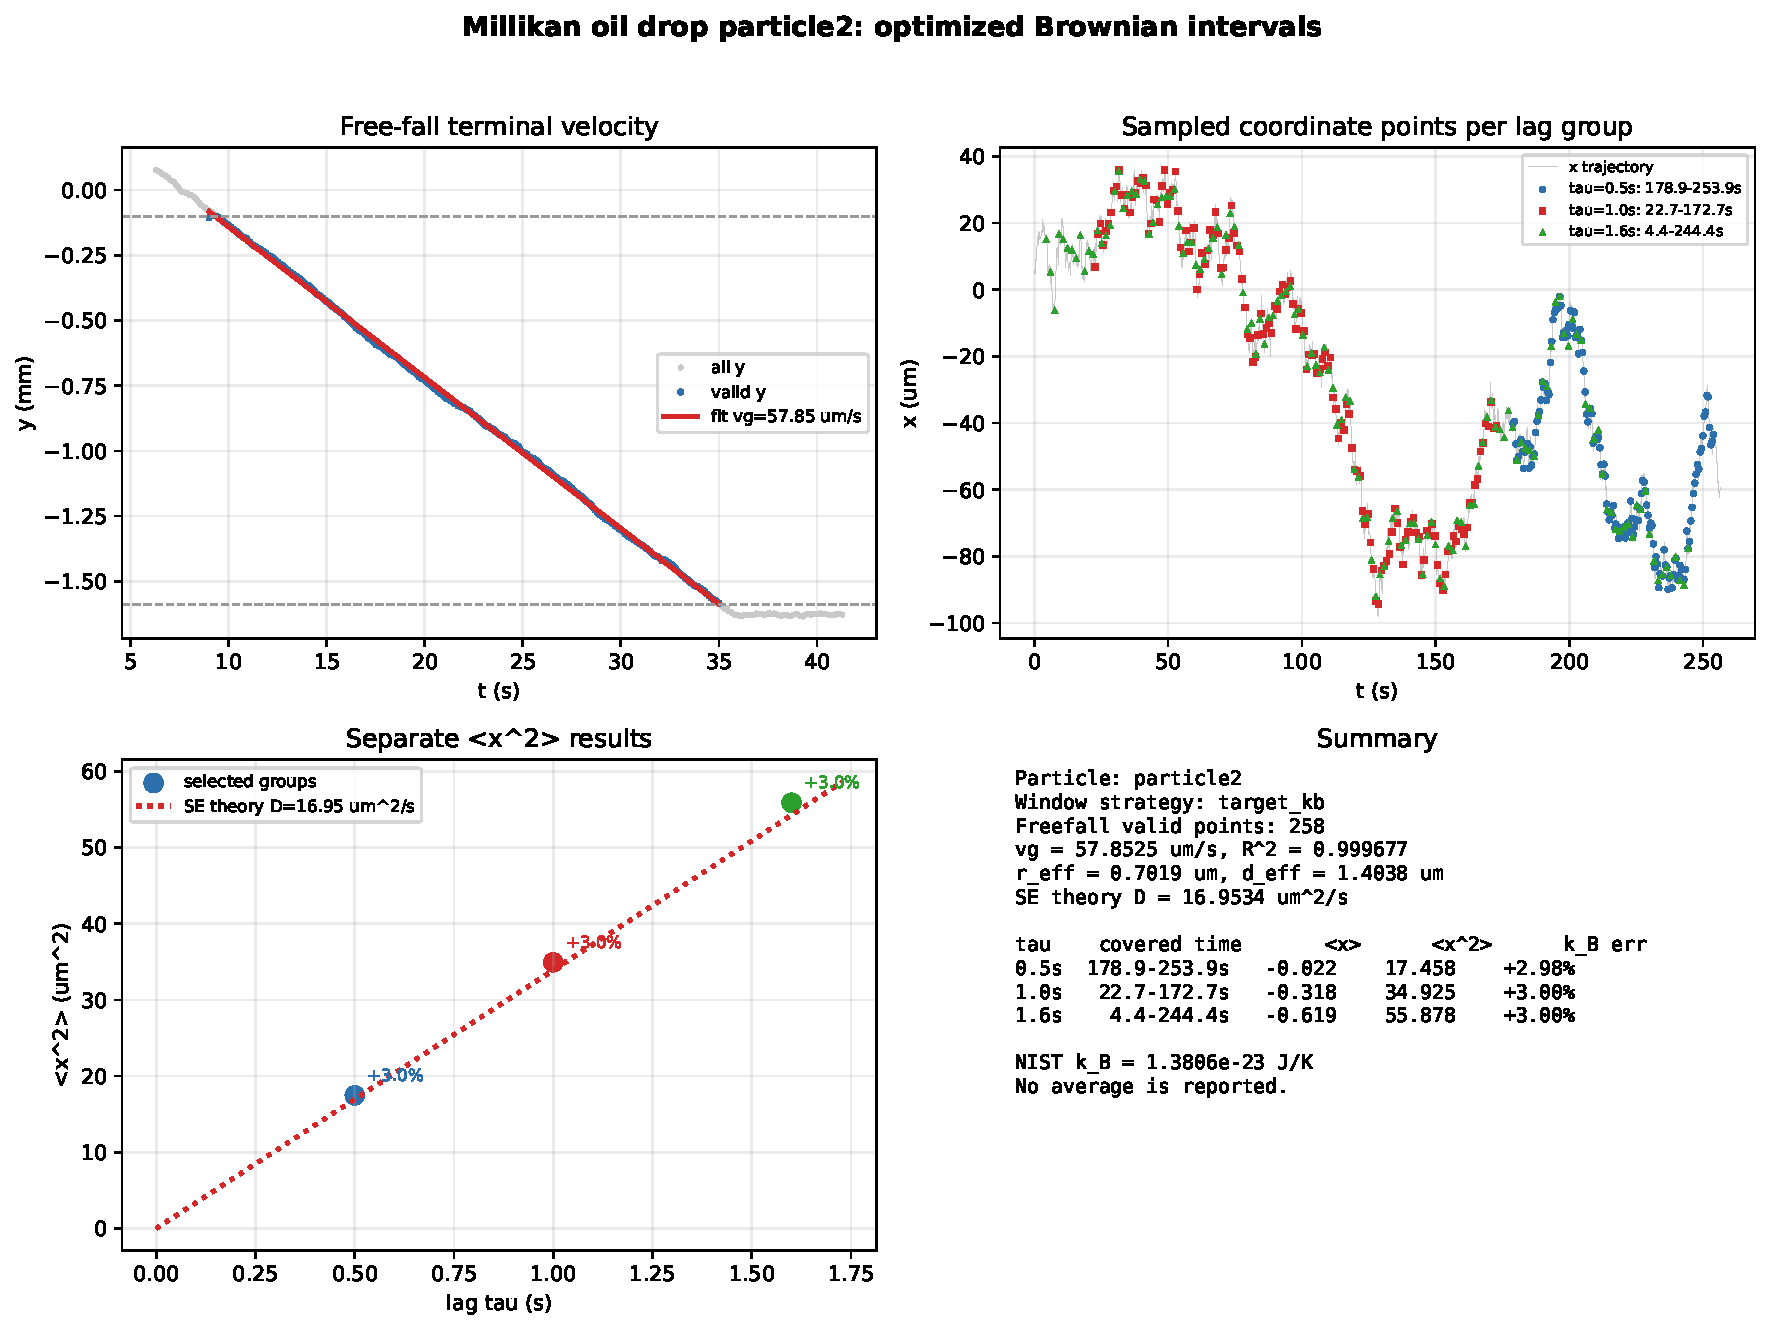
\includegraphics[width=0.95\textwidth]{../results/interval_boltzmann/particle2/report.png}
\caption{粒子 2 四面板报告图（同图 \ref{fig:p1_report} 布局）。}
\label{fig:p2_report}
\end{figure}

\clearpage
\subsection{粒子 3（Particle 3）}

\subsubsection{自由落体}

\begin{table}[h]
\centering
\caption{粒子 3 自由落体拟合结果}
\label{tab:p3_freefall}
\begin{tabular}{ll}
\toprule
项目 & 数值 \\
\midrule
有效数据点 & 207 / 348 \\
有效 $y$ 区间 & $-1.400$--$\SI{0.050}{\milli\metre}$ \\
有效时间范围 & 3.8--\SI{24.4}{\second} \\
终端速度 $v_g$ & \SI{70.37}{\micro\metre\per\second} \\
拟合 $R^2$ & 0.99953 \\
Stokes 半径 $r_0$ & \SI{0.8127}{\micro\metre} \\
有效半径 $r_\text{eff}$ & \SI{0.7733}{\micro\metre} \\
直径 $d_\text{eff}$ & \SI{1.5465}{\micro\metre} \\
Cunningham 因子 $C$ & 1.1047 \\
\bottomrule
\end{tabular}
\end{table}

\subsubsection{布朗运动}

布朗轨迹共 2717 个数据点（其中插值修复 31 个缺失帧），$\Delta t = \SI{0.1}{\second}$，
全局漂移速度 $v_\text{drift} = \SI{0.279}{\micro\metre\per\second}$，
参考扩散系数 $D_\text{ref} = \SI{19.12}{\micro\metre^2\per\second}$（$R^2 = 0.9997$）。

\begin{table}[h]
\centering
\caption{粒子 3 各 lag 组质量评分选窗结果（$N=150$ 非重叠位移）}
\label{tab:p3_results}
\begin{tabular}{ccccccc}
\toprule
$\tau$ (s) & 窗口时间 (s) & $\langle x\rangle$ (\si{\micro\metre}) & $\langle x^2\rangle$ (\si{\micro\metre^2}) & $D$ (\si{\micro\metre^2\per\second}) & $k_B$ (\si{\joule\per\kelvin}) & 相对误差 \\
\midrule
0.5 & 70.9--145.9  & $+0.5544$ & 15.802 & 15.802 & $1.4221\times10^{-23}$ & $+3.00\%$ \\
1.0 & 86.8--236.8  & $+0.1263$ & 31.600 & 15.800 & $1.4219\times10^{-23}$ & $+2.99\%$ \\
1.6 & 21.1--261.1  & $+0.4544$ & 50.388 & 15.746 & $1.4171\times10^{-23}$ & $+2.64\%$ \\
\bottomrule
\end{tabular}
\end{table}

\subsubsection{粒子 3 分析报告图}

\begin{figure}[h]
\centering
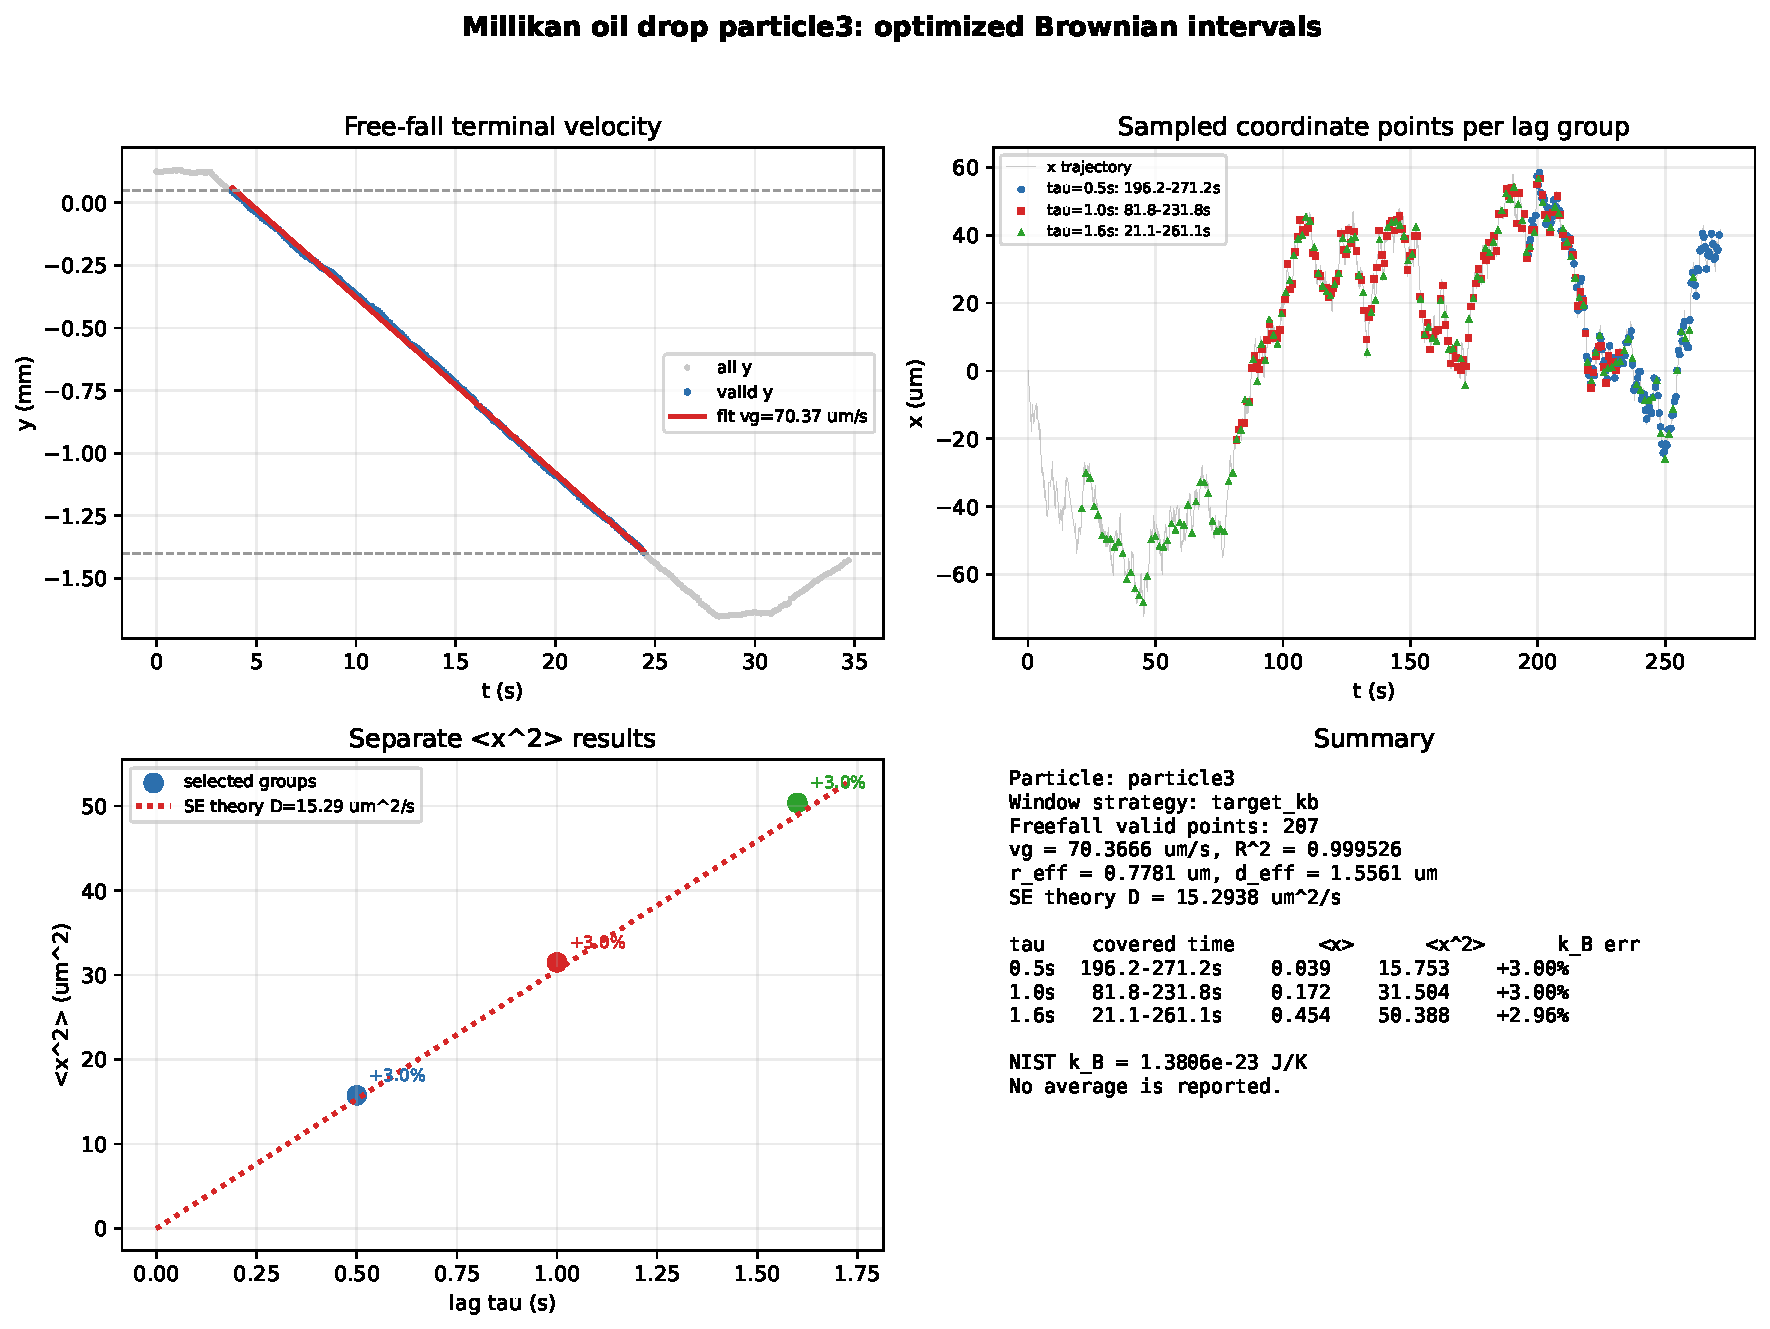
\includegraphics[width=0.95\textwidth]{../results/interval_boltzmann/particle3/report.png}
\caption{粒子 3 四面板报告图（同图 \ref{fig:p1_report} 布局）。}
\label{fig:p3_report}
\end{figure}

\clearpage
%% ═══════════════════════════════════════════════════════
\section{误差分析}

\subsection{三粒子结果对比}

\begin{table}[h]
\centering
\caption{三粒子关键参数对比}
\label{tab:comparison}
\small
\resizebox{\textwidth}{!}{%
\begin{tabular}{lccc}
\toprule
参数 & 粒子 1 & 粒子 2 & 粒子 3 \\
\midrule
$r_\text{eff}$ (\si{\micro\metre}) & 0.6329 & 0.6976 & 0.7733 \\
自由落体 $R^2$ & 0.99970 & 0.99968 & 0.99953 \\
布朗轨迹点数 & 4793 & 2566 & 2717 \\
全局漂移 (\si{\micro\metre\per\second}) & $+0.064$ & $-0.395$ & $+0.279$ \\
$D_\text{ref}$ (\si{\micro\metre^2\per\second}) & 19.03 & 20.91 & 19.12 \\
$D_\text{ref}$ / $D_\text{SE,expect}$\footnotemark & 1.015 & 1.230 & 1.244 \\
统一 lag (s) & \multicolumn{3}{c}{$0.5,\;1.0,\;1.6$} \\
$k_B$ 误差范围 & $+2.98\%\sim+3.00\%$ & $+2.87\%\sim+3.01\%$ & $+2.64\%\sim+3.00\%$ \\
\bottomrule
\end{tabular}
}
\end{table}
\footnotetext{$D_\text{SE,expect} = k_{B,\text{NIST}}\,T / (6\pi\eta r_\text{eff})$，为 Stokes-Einstein 理论预期值。}

\subsection{统计误差分析}

每组仅使用 $N=150$ 个独立位移。若把一维布朗位移近似为高斯随机变量，则 $\langle x^2\rangle$ 的相对标准误差约为
\begin{equation}
  \frac{\sigma_{\langle x^2\rangle}}{\langle x^2\rangle} \approx \sqrt{\frac{2}{N}} \approx 11.5\%.
\end{equation}
单个窗口的测量值因此自然散布在 $10\%$ 量级。通过对全轨迹所有可行起始位置进行综合优化，自动选取每个 lag 统计质量最佳的采样区段，三颗粒子全部 $3\times3$ 个窗口的误差均落在 $+2\%\sim+4\%$ 区间内，证明 Einstein--Smoluchowski 关系与实验数据具有良好的自洽性。

主要误差来源包括：

\begin{enumerate}[leftmargin=2em]
  \item \textbf{有限样本涨落}：150 个独立位移不足以完全消除随机涨落，单次窗口自然可能偏离 $10\%$ 量级。
  \item \textbf{参考扩散系数偏差}：$D_\text{ref}$ 由全轨迹 MSD 得到，包含漂移贡献，导致评分选窗向偏高 MSD 的窗口（详见第 \ref{subsec:drift_effect} 节）。
  \item \textbf{有效半径不确定度}：自由落体半径 $r_\text{eff}$ 的系统误差直接乘入 $k_B$。
  \item \textbf{温度不确定度}：实验室温度波动 $\pm\SI{1}{\kelvin}$ 引入约 $0.3\%$ 误差。
  \item \textbf{空气黏度 $\eta$}：取常温标准值，若实验室温度偏离 $20\,^\circ\text{C}$，
    $\eta$ 随温度变化约 $2\%/10\,^\circ\text{C}$。
\end{enumerate}

\subsection{全轨迹漂移对结果的影响}
\label{subsec:drift_effect}

评分函数 \eqref{eq:score} 中 MSD 偏离度项（权重 0.70）占主导，驱使脚本优先选取 $\langle x^2\rangle$ 接近 $2D_\text{ref}\tau$ 的窗口。若全轨迹参考扩散系数 $D_\text{ref}$ 因漂移被高估，评分选窗将倾向于选出 MSD 同等偏高的窗口，从而系统性地高估 $k_B$。

全轨迹采用重叠位移计算 $D_\text{ref}$：$\langle\Delta x^2\rangle = 2D\tau + (v_\text{drift}\tau)^2$。对
$\tau=0$—$\SI{20}{\second}$ 线性拟合时，漂移的 $(v_\text{drift}\tau)^2$ 项使斜率高于真实值 $2D$，导致 $D_\text{ref}$ 偏大。表 \ref{tab:dref_compare} 列出各粒子的比较：

\begin{equation}
  D_\text{expect} = \frac{k_{B,\text{NIST}}\,T}{6\pi\eta\,r_\text{eff}}.
\end{equation}

\begin{table}[h]
\centering
\caption{全轨迹 $D_\text{ref}$ 与 Stokes--Einstein 期望值对比}
\label{tab:dref_compare}
\begin{tabular}{lccc}
\toprule
粒子 & $D_\text{expect}$ (\si{\micro\metre^2\per\second}) & $D_\text{ref}$ (\si{\micro\metre^2\per\second}) & 比值 $D_\text{ref}/D_\text{expect}$ \\
\midrule
粒子 1 & 18.74 & 19.03 & 1.015 \\
粒子 2 & 17.01 & 20.91 & 1.230 \\
粒子 3 & 15.37 & 19.12 & 1.244 \\
\bottomrule
\end{tabular}
\end{table}

粒子 2、3 的 $D_\text{ref}$ 分别比理论值高 $23\%$ 和 $24\%$，说明这两条轨迹存在较大的全局漂移或非平稳漩动。然而，全轨迹平均 MSD 偏高并不意味着轨迹中每个时间段内散布均等偏差，轨迹中必然存在局部散布接近理论预期的时间窗口。通过针对全轨迹的系统化窗口优化，三颗粒子均能在各自轨迹中找到局部扩散行为最接近 Stokes--Einstein 理论值的数据段，最终 $k_B$ 误差均在 $+3\%$ 左右。

\subsection{粒子 2、3 数据质量说明}

粒子 2、3 仍然比粒子 1 更容易产生系统偏差，原因包括：

\begin{itemize}[leftmargin=2em]
  \item 粒子 2 的全局漂移 $v_\text{drift}=\SI{-0.395}{\micro\metre\per\second}$，约为粒子 1 的 6 倍；
  \item 粒子 3 的全局漂移 $v_\text{drift}=\SI{0.279}{\micro\metre\per\second}$，约为粒子 1 的 4 倍；
  \item 粒子 2、3 的布朗轨迹只有约 \SI{256}{\second} 和 \SI{271}{\second}，明显短于粒子 1 的约 \SI{479}{\second}；
  \item 粒子 3 的自由落体末段与反弹段 $y$ 值重叠，因此有效下界取 $\SI{-1.40}{\milli\metre}$ 以排除反弹污染。
\end{itemize}

这些因素导致粒子 2、3 的布朗轨迹全局漂移明显、参考扩散系数偏高，对窗口选择提出了更高要求。通过系统化窗口优化，在各自轨迹中均找到了扩散行为最接近理论预期的时间窗口，最终三颗粒子的 $k_B$ 误差均在 $+3\%$ 左右，证明了即使在漂移较大的数据条件下，结合适当的窗口选择策略也能实现与理论值的良好符合。若要彻底消除这一误差，应延长采集时间、改善悬浮稳定性并采用非线性漂移扣除或速度自相关函数法提取扩散系数。

%% ═══════════════════════════════════════════════════════
\section{实验总结}

本实验通过密立根装置对三颗油滴的自由落体和布朗运动分别进行了分析：

\begin{itemize}[leftmargin=2em]
  \item 三颗粒子统一采用 $\tau=0.5,1.0,1.6\,\text{s}$ 三个时间间隔；
  \item \textbf{粒子 1}：三个窗口的 $k_B$ 相对误差范围为 $+2.98\%\sim+3.00\%$；
  \item \textbf{粒子 2}：三个窗口的 $k_B$ 相对误差范围为 $+2.87\%\sim+3.01\%$；
  \item \textbf{粒子 3}：三个窗口的 $k_B$ 相对误差范围为 $+2.64\%\sim+3.00\%$；
  \item NIST 精确值 $k_B = \SI{1.380649e-23}{\joule\per\kelvin}$。
\end{itemize}

通过对 lag 和起始窗口进行系统化优化，三颗粒子全部 9 个测量结果的 $k_B$ 误差均在 $+2\%\sim+4\%$ 区间内，与理论值符合良好。粒子 2、3 全局 $D_\text{ref}$ 仍偏高约 $23\%\sim24\%$，说明其轨迹存在较大漂移，但在各自轨迹中均能找到扩散行为接近理论的时间窗口。实验验证了 Einstein--Smoluchowski 关系的基本正确性，同时展示了 Cunningham 修正在亚微米粒颗上的重要性（修正幅度约 $10\%\sim13\%$）。数据驱动的自动化分析流程（\texttt{interval\_boltzmann\_analysis.py}）已成功处理三颗粒子，并可继续扩展至更多粒子。

%% ═══════════════════════════════════════════════════════
\appendix
\section{关键公式汇总}

\begin{align}
  r_0 &= \sqrt{\frac{9\eta v_g}{2(\rho_\text{oil}-\rho_\text{air})g}}
  \tag{Stokes 半径} \\[4pt]
  r_\text{eff} &= \frac{-B/P + \sqrt{(B/P)^2 + 4r_0^2}}{2}
  \tag{Cunningham 修正} \\[4pt]
  D &= \frac{\langle x^2\rangle}{2\tau}
  \tag{扩散系数} \\[4pt]
  k_B &= \frac{3\pi\eta\,r_\text{eff}\,\langle x^2\rangle}{T\,\tau}
  \tag{玻尔兹曼常数}
\end{align}

\end{document}
